\section{Backend-Logik}

Die Logik des Feasibility-Check-Algorithmus besteht aus vier zentralen Methoden, die zusammen die Prüfung der Machbarkeit eines Tests realisieren. Zum einen gibt es eine Helfer-Methode, die den eigentlichen Algorithmus aufruft und sicherstellt, dass der Aufrufer der REST-API eine aussagekräftige Rückmeldung erhält. Die Kernkomponente bildet die \texttt{FeasibilityCheck()}-Methode, welche abhängig von der Art der Überprüfung den Condition oder den Equipment Check aufruft. Beide Prüfungen sind als eigenständige Methoden implementiert. Der gesamte Ablauf wird durch vier Aktivitäts- bzw. Flussdiagramme visualisiert. In diesen Diagrammen werden Schleifen durch farblich hervorgehobene Bereiche dargestellt, die jeweils einen gleichfarbigen Kreis als Einstiegspunkt sowie einen zweiten als Ausstiegspunkt enthalten.

Die Ausführung des Algorithmus wird initiiert, sobald der Benutzer im Frontend einen \textit{Button} in der Weboberfläche betätigt. Dies löst einen asynchronen HTTP-Call über eine REST-API aus, welcher die Helfer-Methode \texttt{CheckFeasibility()} aufruft und die Test-ID des zu überprüfenden Tests als Argument übergibt.

\begin{figure}[!htbp]
    \centering
    \makebox[\textwidth]{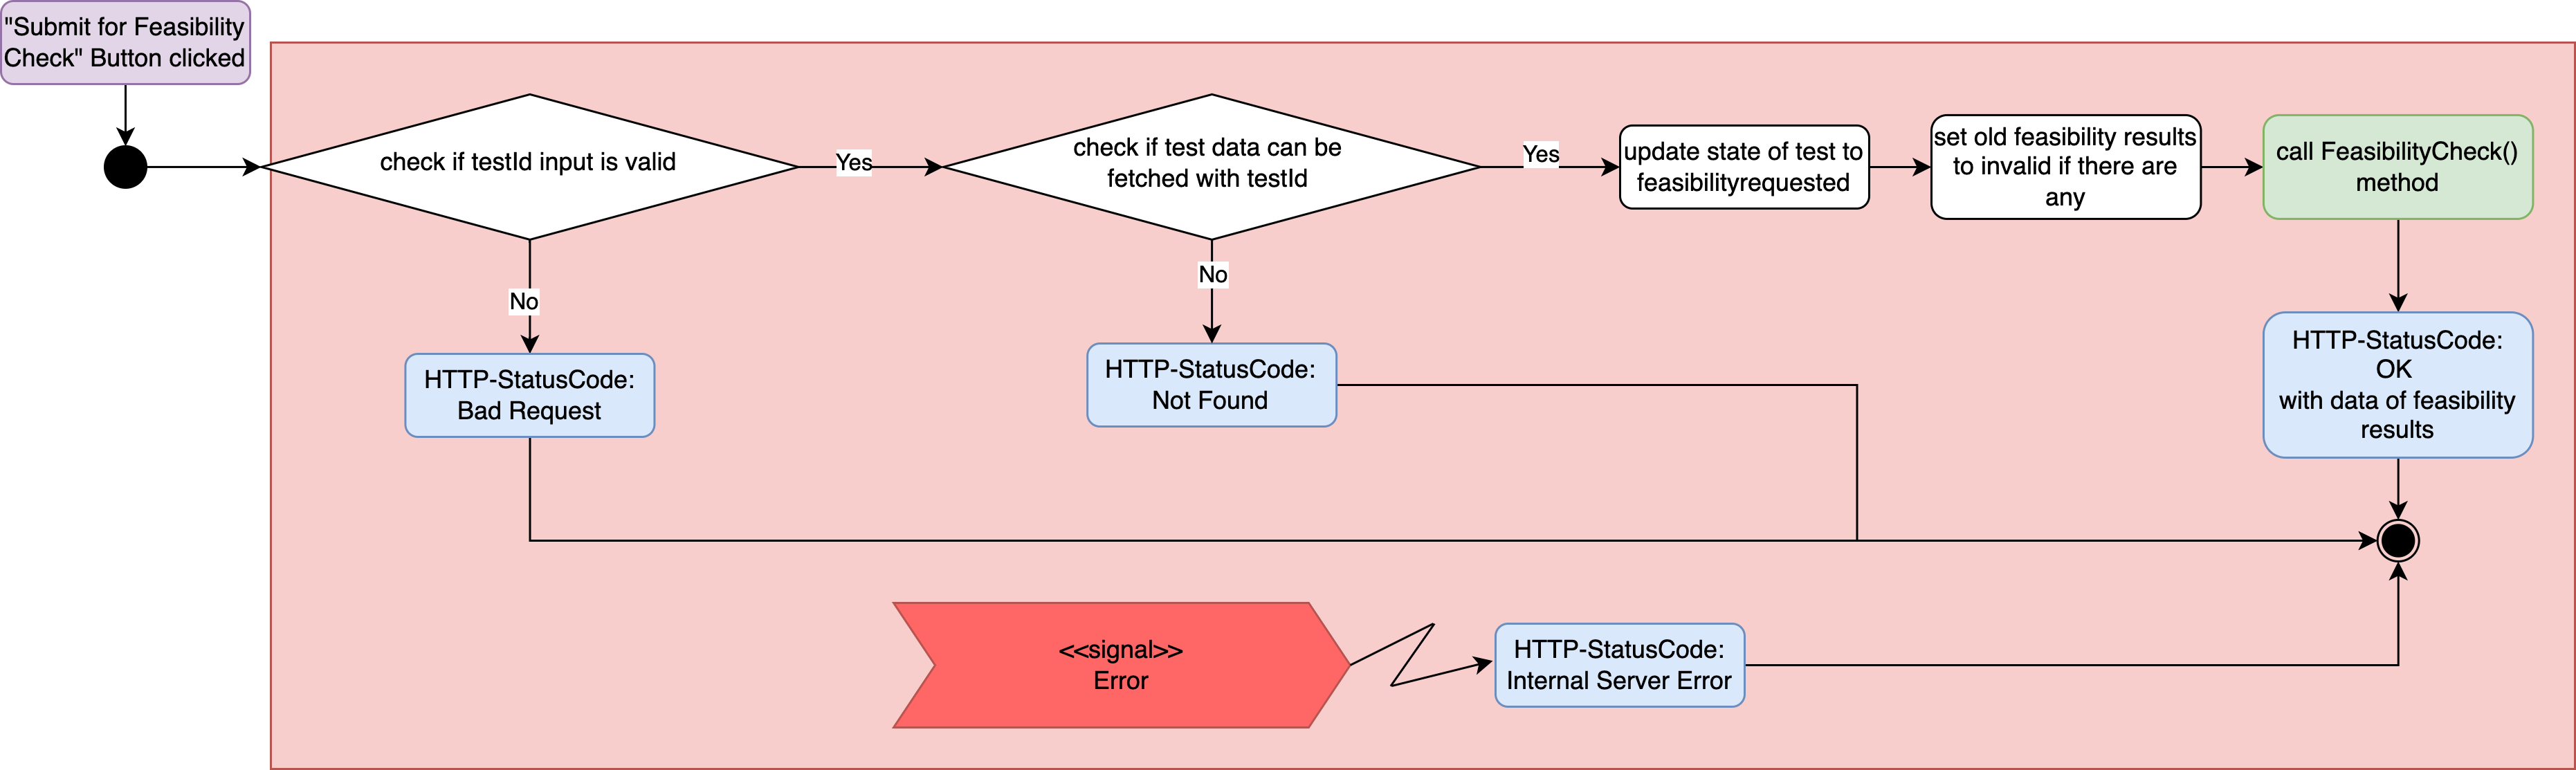
\includegraphics[width=0.85\paperwidth]{bilder/flowchart-check-feasibility-http-call-6-2.png}}
    \caption{Flussdiagramm der Helfer-Methode \texttt{CheckFeasibility()}}
    \label{fig:feasibility-http-call-method}
\end{figure}

Der Ablauf dieser Helfer-Methode ist in Abbildung \ref{fig:feasibility-http-call-method} dargestellt. Ihre Hauptaufgabe besteht darin, die eigentliche \texttt{FeasibilityCheck()}-Methode (grünes Rechteck in der Graphik \ref{fig:feasibility-http-call-method}) auszuführen und gleichzeitig eine geeignete HTTP-Statusmeldung an das Frontend bzw. den Benutzer zurückzugeben. Zusätzlich wird vor der Verarbeitung die übergebene Test-ID auf Gültigkeit überprüft und der Test-Status aktualisiert. Falls der FeasibilityCheck für diesen Test bereits zuvor durchgeführt wurde, werden alte Ergebnisse in der Datenbank als ''invalid'' markiert.


Zur besseren Übersicht wird in Abbildung \ref{fig:feasibility-http-call-method} auch der initiale Button-Klick im Frontend als Aktivität dargestellt. Die eigentliche Logik beginnt jedoch erst nach dem schwarzen Einstiegspunkt, der den Start des Algorithmus kennzeichnet.

\begin{figure}[!htbp]
    \centering
    \makebox[\textwidth]{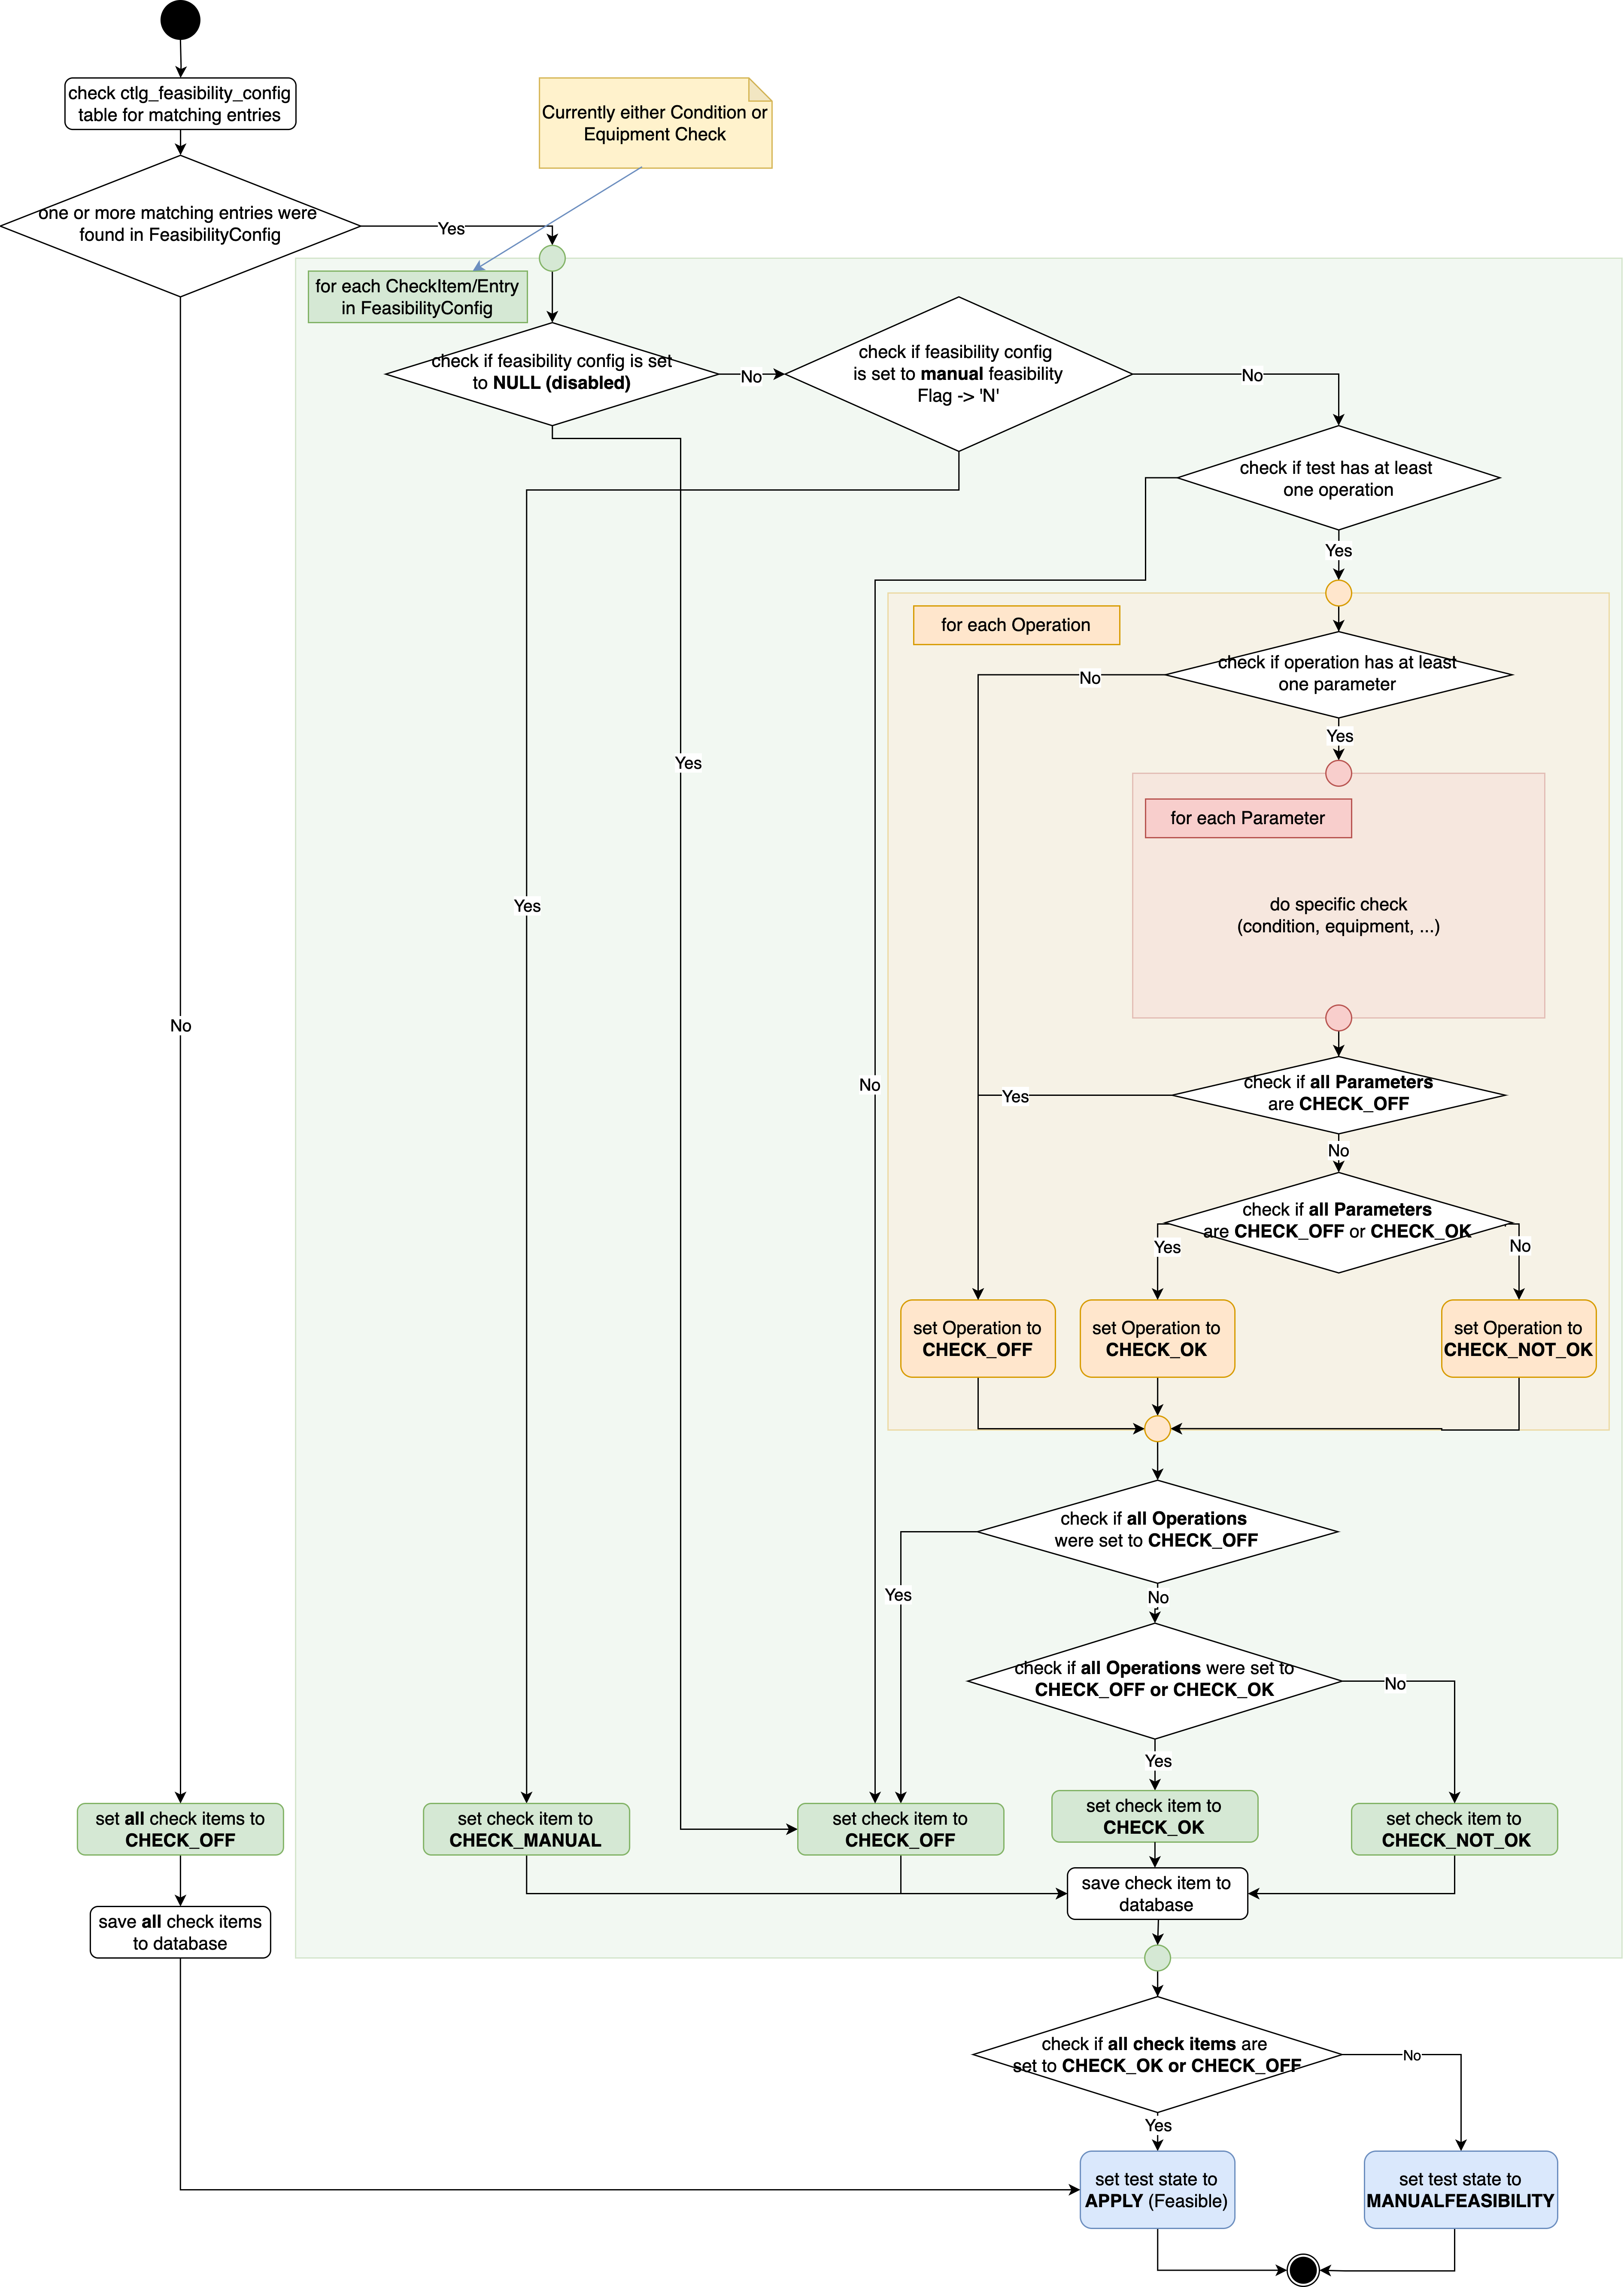
\includegraphics[width=0.85\paperwidth]{bilder/flowchart-feasibilitycheck-modiefied-for-thesis-6-2.png}}
    \caption{Flussdiagramm des Feasibility Check}
    \label{fig:feasibility-check}
\end{figure}

Die Kernlogik des Feasibility Checks wird durch die Methode \texttt{FeasibilityCheck()} ausgeführt, die im Flussdiagramm in Abbildung \ref{fig:feasibility-check} detailliert dargestellt ist. Diese Methode erhält von der Helfer-Methode die Test-ID und überprüft die Machbarkeit des Tests anhand der relevanten Parameter und Operationen. Um die Logik des Algorithmus zu vereinfachen, wird ein Enum eingeführt, das den Status einzelner \textit{Teil-Checks} kennzeichnet. Dieser besteht aus vier möglichen Stati mit jeweils spezifischer Bedeutung:

\setlength{\leftskip}{1em}
\textbf{\texttt{CHECK\_OFF}} - Der Check ist deaktiviert; eine Überprüfung ist weder erforderlich noch vorgesehen. Dies ist insbesondere der Fall, wenn ein Parameter bzw. eine Operation keine Stressoperation darstellt und somit keine PlanValue definiert werden muss.

\textbf{\texttt{CHECK\_OK}} - Der Check war erfolgreich.

\textbf{\texttt{CHECK\_NOT\_OK}} - Der Check war nicht erfolgreich oder es ist ein Fehler aufgetreten.

\textbf{\texttt{CHECK\_MANUAL}} - Eine automatische Überprüfung ist nicht möglich oder der Check ist noch nicht für die automatisierte Überprüfung zugelassen; der Check muss von einem Mitarbeiter manuell durchgeführt werden.

\setlength{\leftskip}{0em} 

Jeder Parameter-Überprüfung wird einer dieser vier Stati zugewiesen. Anschließend wird basierend auf den Statuswerten der einzelnen Parameter ein Gesamtstatus für die zugehörige Operation ermittelt (siehe orange markierte Aktivitäten in Abb. \ref{fig:feasibility-check}). Die Stati aller Operationen ergeben wiederum einen Gesamtstatus für das jeweilige \textit{CheckItem} (\gls{ConditionCheck} oder \gls{EquipmentCheck}) (grüne Aktionen). Dieses Ergebnis dieser Überprüfung wird anschließend als \texttt{feasibility\_check\_item\_result} in der Datenbank gespeichert.

Da die Mehrheit der Ergebnisse den Status \texttt{CHECK\_OFF} aufweist, werden diese nicht in der Datenbank gespeichert, um eine unnötige Datenaufblähung zu vermeiden. Zudem würden in solchen Fällen keine zusätzlichen, für den Benutzer relevanten Informationen generiert werden, da der Status lediglich siganlisiert, dass der Test nicht detailliert überprüft wurde – entweder weil er deaktiviert ist oder weil er keine Operation enthält.

Schließlich wird auf Basis aller \textit{CheckItem}-Ergebnisse der finale Test-Status ermittelt (blaue Aktivitäten). Dieser kann entweder \textbf{''FEASIBLE''} („APPLY“; erfolgreich) oder \textbf{''MANUAL\_FEASIBLE''} (manuelle Überprüfung erforderlich) sein.

Um es zu ermöglichen, dass bestimmte \textit{CheckItems} für einen Test in der Konfiguration vollständig deaktiviert werden können – wobei dies im System als erfolgreiche Überprüfung gewertet wird – kann das entsprechende Flag in der Feasibility-Konfiguration entweder leer (\textit{null}) gelassen werden oder es wird für das betreffende CheckItem gar kein Eintrag in der Konfigurations-Tabelle erstellt. \todo{Beispiel}

\textbf{Konkreter Ablauf des Feasibility Check Algorithmus} \\
Zunächst werden die für den Test hinterlegten Konfigurationen für jedes \texttt{CheckItem} aus der Datenbank abgerufen. Falls kein Eintrag existiert, wird der Check automatisch als erfolgreich gewertet. Ist das zugehörige Flag auf 'N' gesetzt, muss die Überprüfung manuell erfolgen, und der Check ist an dieser Stelle beendet. Nur wenn das Flag auf 'Y' gesetzt ist, wird das entsprechende \textit{CheckItem} (Condition oder \gls{EquipmentCheck}) tatsächlich geprüft.

Anschließend wird überprüft, ob der Test mindestens eine Operation enthält. Falls ja, wird jede dieser Operationen durchlaufen, um festzustellen, ob sie einen oder mehrere Parameter besitzt. Für jeden Parameter wird dann – abhängig vom \textit{CheckItem} – entweder der \gls{ConditionCheck} oder der \gls{EquipmentCheck} durchgeführt.

\subsection{Condition Check}

\begin{figure}[!htbp]
    \centering
    \makebox[\textwidth]{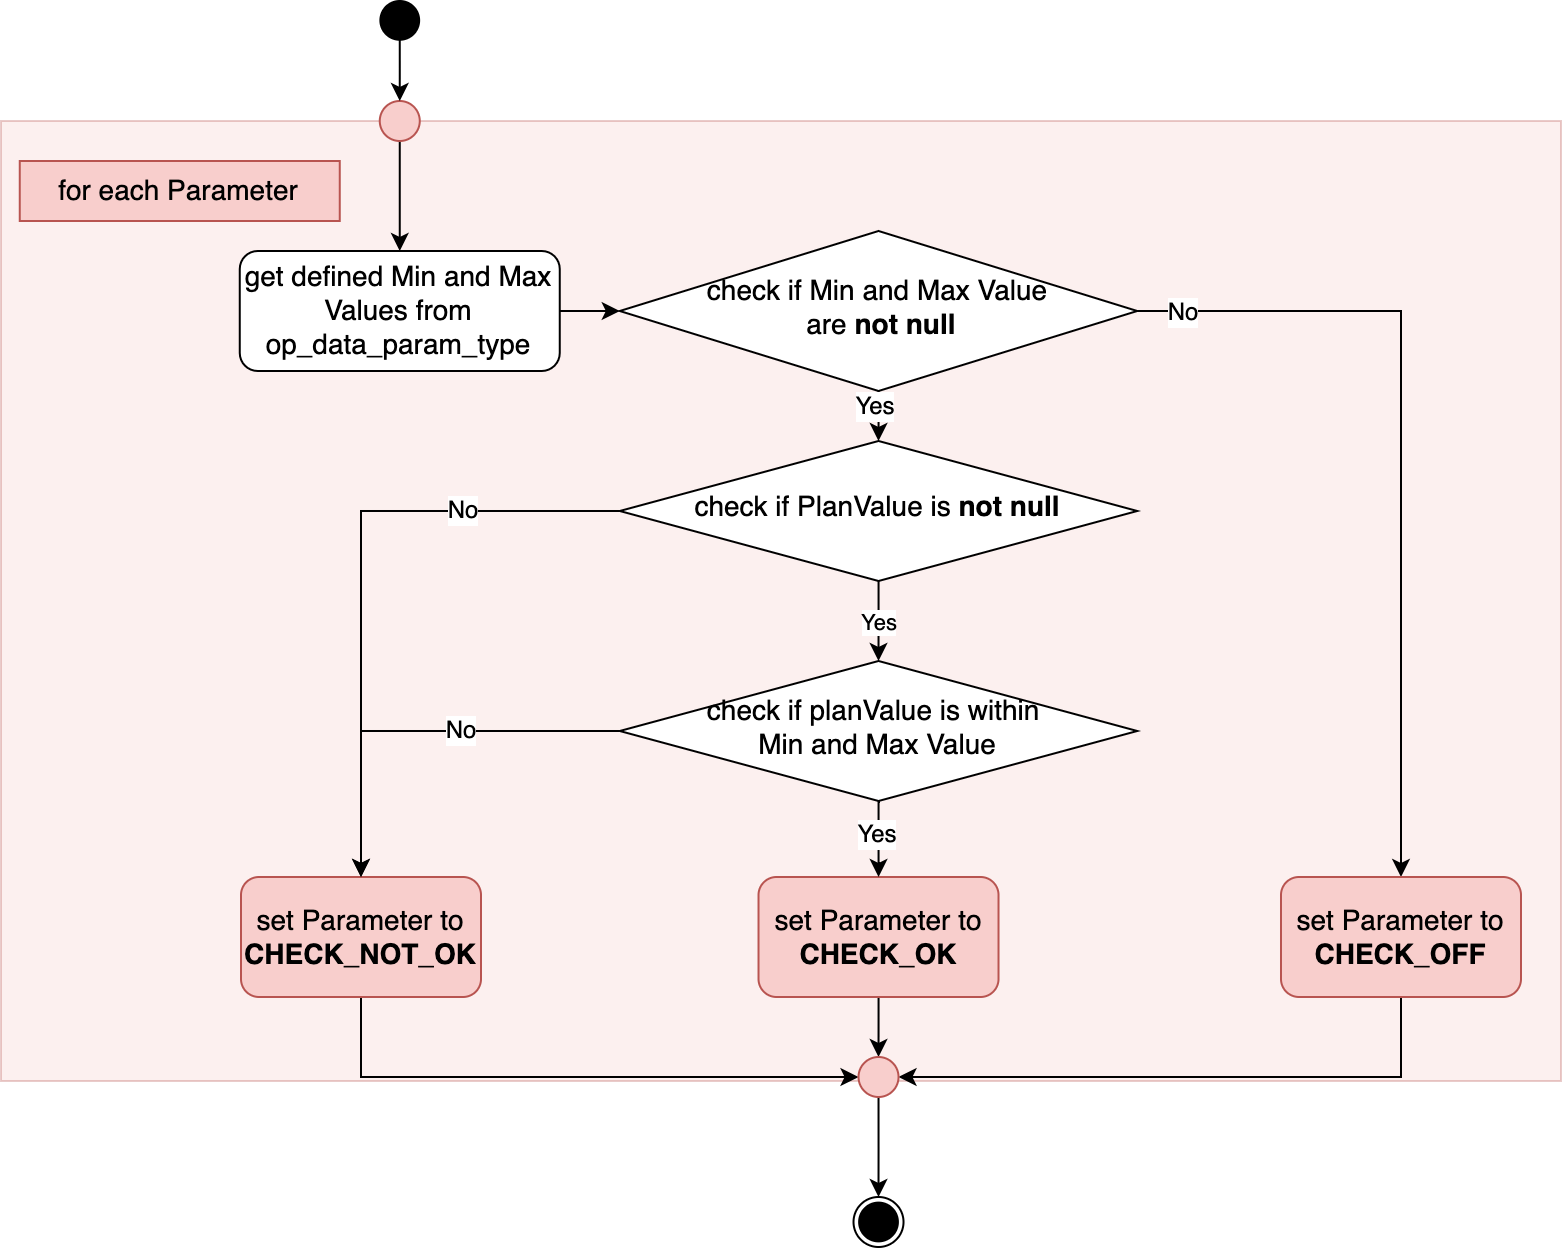
\includegraphics[width=0.80\paperwidth]{bilder/flowchart-condition-check-6-2.png}}
    \caption{Flussdiagramm des \gls{ConditionCheck}s}
    \label{fig:condition-check}
\end{figure}

Der Ablauf des \gls{ConditionCheck} ist in Abbildung \ref{fig:condition-check} dargestellt. Zunächst wird die relevante Verknüpfungstabelle \texttt{op\_data\_param\_type} aus der Datenbank abgerufen. Diese Tabelle definiert den zulässigen Wertebereich eines Parameters durch einen minimalen und maximalen Wert. Falls weder ein minimaler noch ein maximaler Wert definiert ist, wird der \textit{Parameter-Teil-Check} auf \texttt{CHECK\_OFF} gesetzt, was bedeutet, dass keine Überprüfung erforderlich ist und der Parameter automatisch als gültig betrachtet wird. Sind sowohl ein minimaler als auch ein maximaler Wert hinterlegt, muss zusätzlich ein geplanter Wert (\textit{PlanValue}) für den Parameter vorhanden sein. Liegt dieser innerhalb des zulässigen Bereichs, gilt die Sinnhaftigkeitsprüfung als erfolgreich, und der nächste Parameter der Operation wird verarbeitet.


Falls nur ein Mindest- oder Höchstwert in der Datenbank definiert ist, genügt es, wenn der \textit{PlanValue} entweder über dem Mindestwert oder unter dem Höchstwert liegt. Diese Sonderfälle sind zur besseren Übersichtlichkeit nicht im Flussdiagramm \ref{fig:condition-check} dargestellt.




\subsection{Equipment Check}
Der \gls{EquipmentCheck} ist in Abbildung \ref{fig:equipment-check} dargestellt. Der Prozess beginnt ebenfalls mit dem Abruf von Daten aus der passenden \texttt{op\_data\_param\_type} Tabelle. Falls keine Referenzen für den minimalen und maximalen Maschinenparameter (\texttt{ctlg\_factsheet\_parameter}) hinterlegt sind, ist die Überprüfung für diese Parameter, nicht erforderlich und ist somit beendet. Andernfalls muss sichergestellt werden, dass ein \textit{PlanValue} gesetzt ist. Erst danach startet der eigentliche Durchführbarkeits-Check.

Als erstes werden aus der Datenbank alle Maschinen abgerufen, die als ''valide'' gelten, also weder defekt noch in Wartung sind, und zudem den gleichen Testsubtypen aufweisen wie der zu prüfende Test. Die Zuordnung der Maschinen zu einem spezifischen Testsubtyp erfolgt dabei indirekt über die Verknüpfungstabelle \texttt{machine\_test\_sub\_type}, welche die Maschinen mit dem jeweiligen \texttt{ctlg\_test\_sub\_type} verknüpft.

Anschließend werden die verbleibenden Maschinen einzeln durchlaufen (siehe lila markierter Bereich in Abbildung \ref{fig:equipment-check}). Zuerst wird analysiert, ob die Maschine im geplanten Zeitraum der Operation zur Verfügung steht. Danach erfolgt die Überprüfung, ob die Maschine den Parameter grundsätzlich umsetzen kann. Dazu wird geprüft, ob die Maschine über die gleichen \texttt{ctlg\_factsheet\_parameter} verfügt, die in der Verknüpfungstabelle definiert sind. Falls dies der Fall ist, werden die minimalen und maximalen Werte über den zugehörigen Eintrag im Maschinen-Factsheet (\texttt{MFS\_VALUE}) abgerufen. Anschließend wird kontrolliert, ob der geplante Wert (\textit{PlanValue}) des Parameters innerhalb dieser Grenzen liegt. Ist dies der Fall, gilt die Maschine als geeignet, den geplanten Wert umzusetzen, und der Equipment-Check wird als erfolgreich betrachtet.

Alle Maschinen, die den Parameter mit dem geplanten Wert umsetzten können, werden in einer Liste als \texttt{check\_item\_result\_list} erfasst und mit dem zugehörigen \texttt{feasibility\_check\_item\_result} später in der Datenbank abgespeichert. 

\begin{figure}[!htbp]
    \centering
    \makebox[\textwidth]{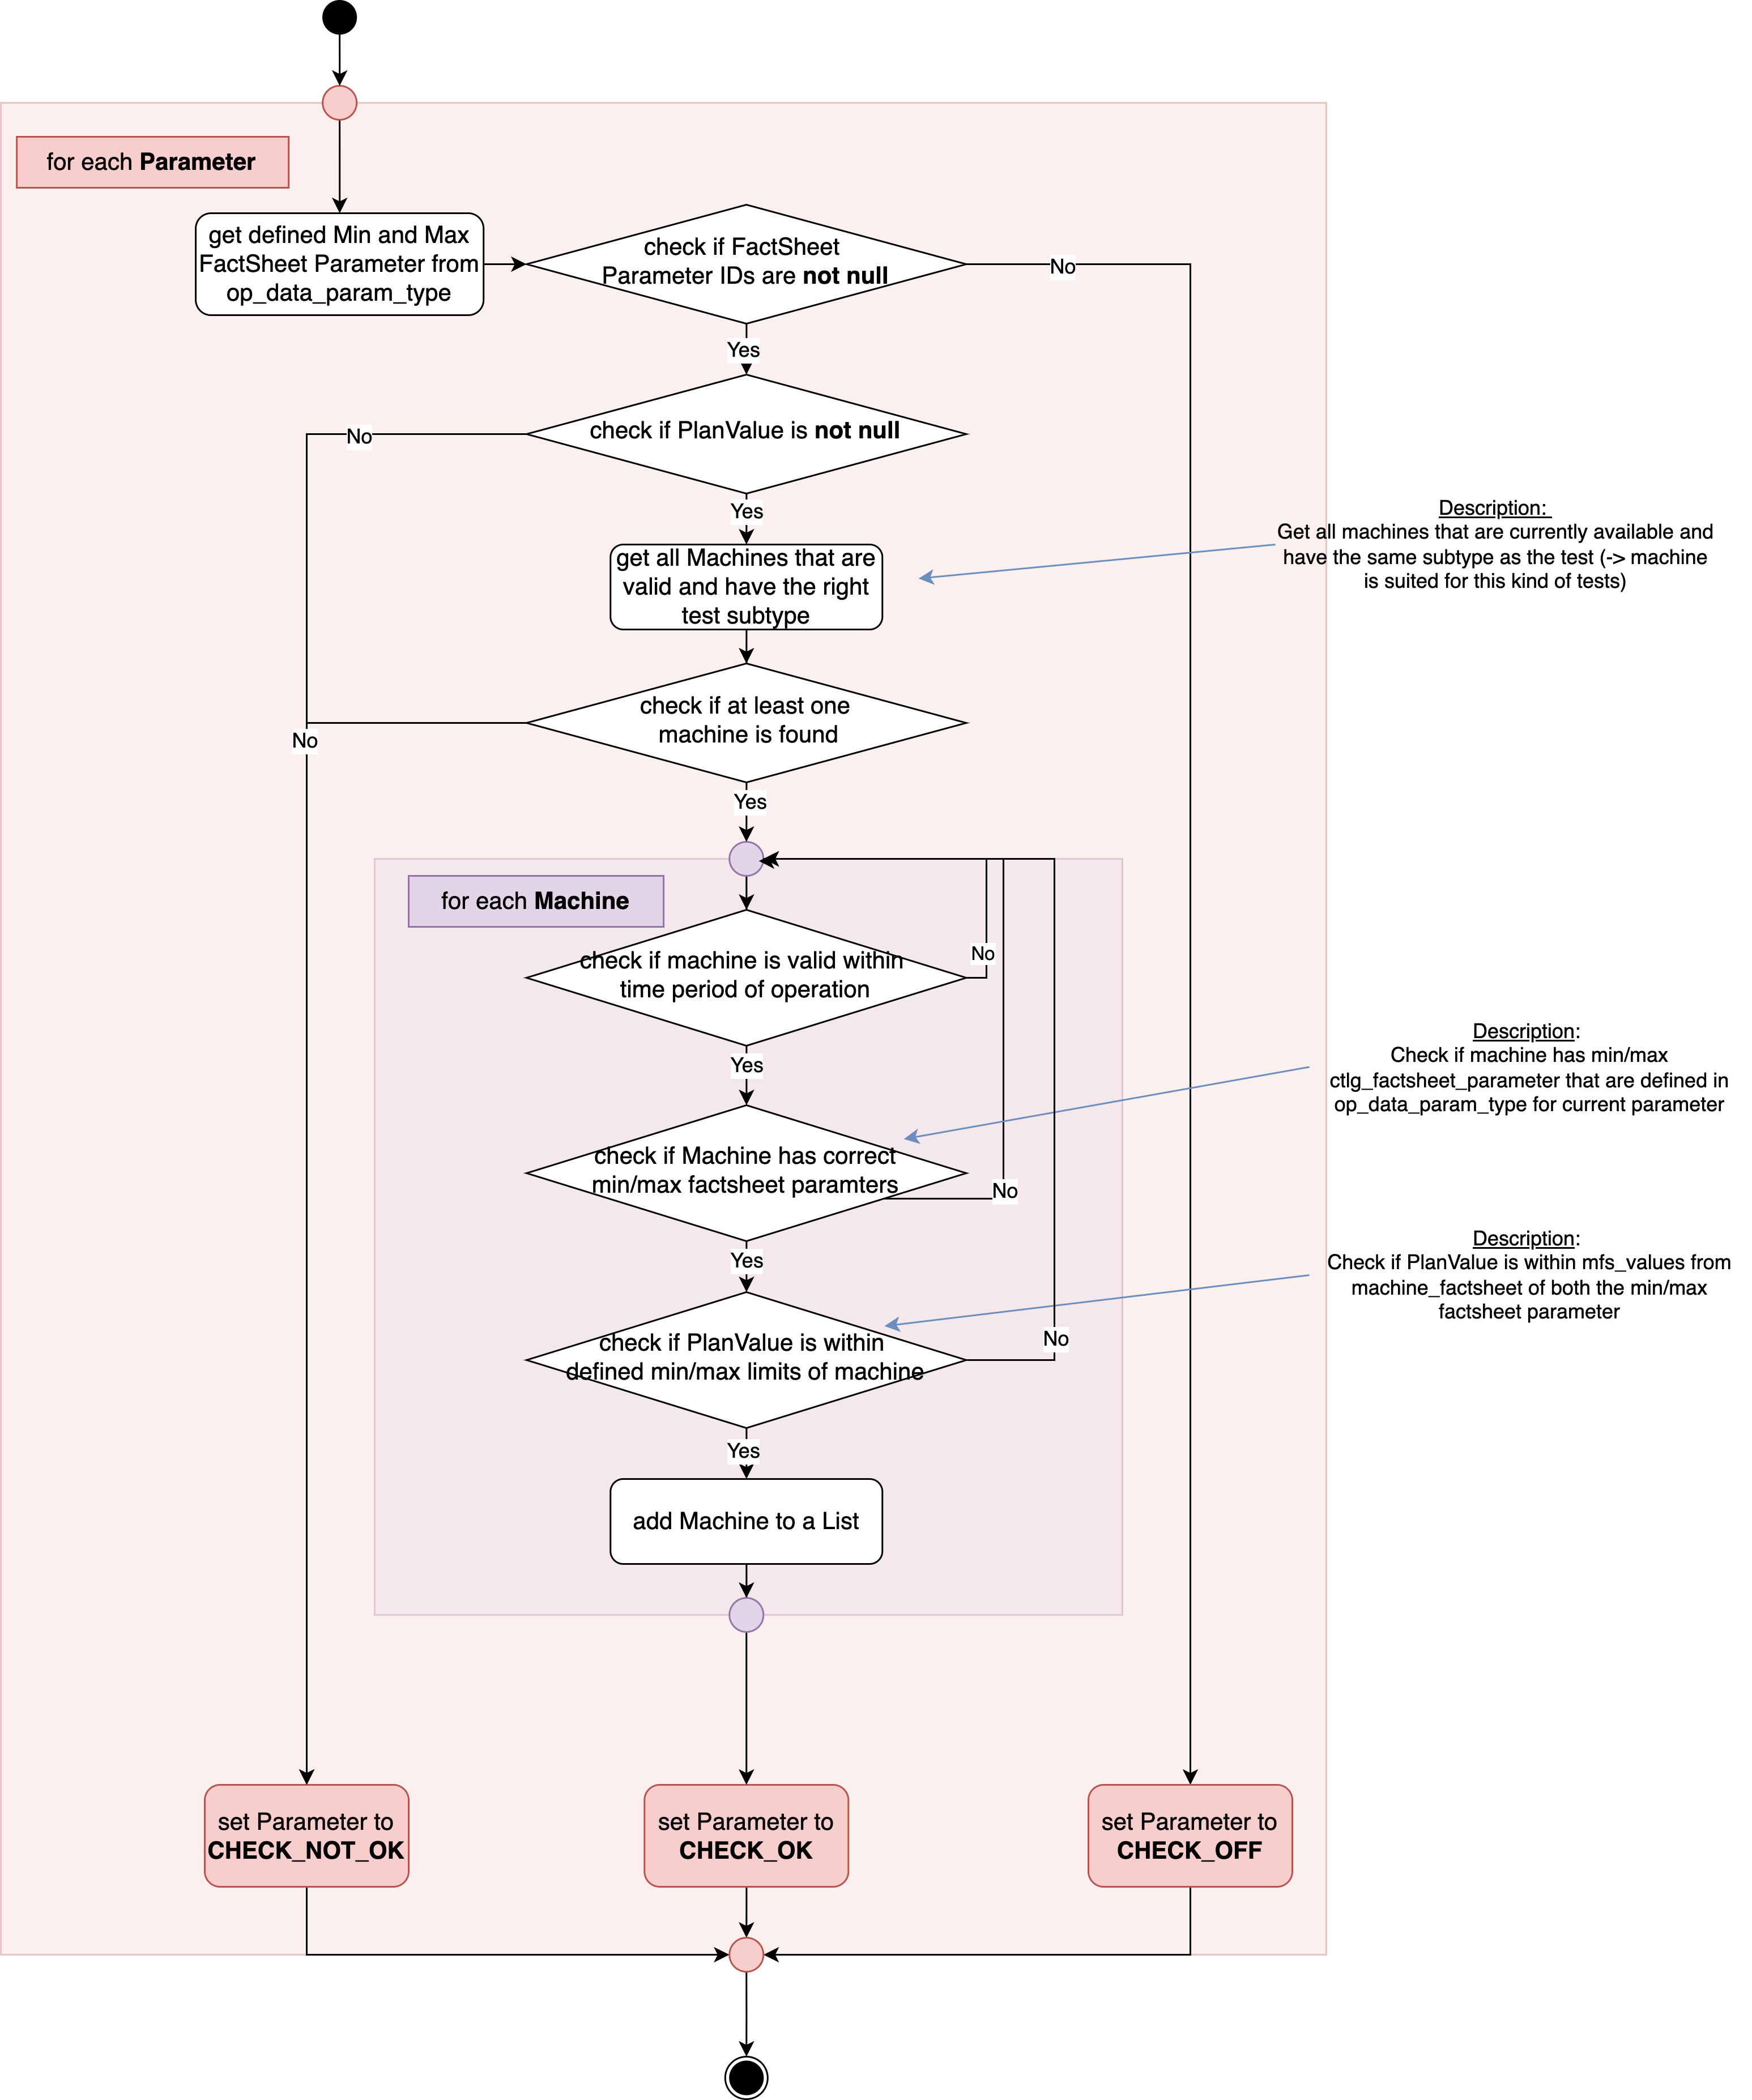
\includegraphics[width=0.85\paperwidth]{bilder/flowchart-equipment-check-6-2.png}}
    \caption{Flowchart des \gls{EquipmentCheck}s}
    \label{fig:equipment-check}
\end{figure}